%% Compile: pdflatex > pdflatex
%% Final thesis presentation, built from thesisv4.tex and generated results tables.

\documentclass[aspectratio=169, 11pt]{beamer}

\usepackage[utf8]{inputenc}
\usepackage[T1]{fontenc}
\usepackage{textcomp}
\usepackage{lmodern}
\usepackage[british]{babel}

\usepackage{amsmath,amssymb}
\usepackage{booktabs}
\usepackage{array}
\usepackage{graphicx}
\usepackage{tikz}
\usetikzlibrary{positioning, arrows, calc, shapes.geometric,
  fit, backgrounds, decorations.pathreplacing, decorations.pathmorphing}
\usepackage{pgfpages}

\definecolor{Navy}{HTML}{0D1B2A}
\definecolor{MidNavy}{HTML}{1B2E4A}
\definecolor{DkOrange}{HTML}{D97706}
\definecolor{LtOrange}{HTML}{F5DEB3}
\definecolor{Bordeaux}{HTML}{7A1C2E}
\definecolor{BordeauxLt}{HTML}{A63D50}
\definecolor{Ivory}{HTML}{FAF8F5}
\definecolor{WarmGrey}{HTML}{E8E4DF}
\definecolor{MidGrey}{HTML}{9CA3AF}
\definecolor{DkGrey}{HTML}{4B5563}
\definecolor{Teal}{HTML}{2A7F8C}
\definecolor{TealLt}{HTML}{D0ECF0}
\definecolor{ForestGreen}{HTML}{4A7C59}
\definecolor{DeepRed}{HTML}{C44536}

\usefonttheme{professionalfonts}
\setbeamercolor{normal text}{fg=Navy, bg=Ivory}
\setbeamercolor{alerted text}{fg=Bordeaux}
\setbeamercolor{example text}{fg=DkOrange}

% Frame title
\setbeamercolor{frametitle}{fg=Ivory, bg=Navy}
\setbeamerfont{frametitle}{size=\large, series=\bfseries}
\setbeamertemplate{frametitle}{%
  \nointerlineskip
  \begin{beamercolorbox}[wd=\paperwidth, ht=2.6em, dp=0.8em, leftskip=1.2em]{frametitle}%
    \usebeamerfont{frametitle}\insertframetitle%
  \end{beamercolorbox}%
  {\color{DkOrange}\hrule height 2.2pt}%
}

% Title page
\setbeamercolor{title}{fg=Ivory}
\setbeamercolor{subtitle}{fg=LtOrange}
\setbeamercolor{author}{fg=Ivory}
\setbeamercolor{date}{fg=WarmGrey}
\setbeamercolor{institute}{fg=WarmGrey}
\setbeamerfont{title}{size=\Large, series=\bfseries}
\setbeamerfont{subtitle}{size=\normalsize, shape=\itshape}

% Itemize
\setbeamertemplate{itemize item}{\color{DkOrange}\scriptsize$\blacksquare$}
\setbeamertemplate{itemize subitem}{\color{Bordeaux}\scriptsize$\blacktriangleright$}
\setbeamercolor{itemize item}{fg=DkOrange}
\setbeamercolor{itemize subitem}{fg=Bordeaux}

% Footer
\setbeamertemplate{navigation symbols}{}
\setbeamertemplate{footline}{%
  \hfill
  \raisebox{3pt}{\color{MidGrey}\scriptsize\insertframenumber\,/\,\inserttotalframenumber}%
  \hspace{8pt}\vspace{3pt}%
}

% Blocks
\setbeamercolor{block title}{fg=Ivory, bg=MidNavy}
\setbeamercolor{block body}{fg=Navy, bg=WarmGrey}
\setbeamercolor{block title alerted}{fg=Ivory, bg=Bordeaux}
\setbeamercolor{block body alerted}{fg=Navy, bg=WarmGrey}
\setbeamercolor{block title example}{fg=Ivory, bg=DkOrange}
\setbeamercolor{block body example}{fg=Navy, bg=WarmGrey}
\setbeamerfont{block title}{series=\bfseries}

\AtBeginSection[]{}

\newcommand{\highlight}[1]{\textcolor{DkOrange}{\textbf{#1}}}
\newcommand{\emphbx}[1]{\textcolor{Bordeaux}{\textbf{#1}}}
\newcommand{\EUR}{\texteuro}
\newcommand{\USD}{US\$}
\newcommand{\pp}{\text{pp}}
\newcommand{\sourceline}[1]{}

\newcolumntype{L}[1]{>{\raggedright\arraybackslash}p{#1}}
\newcolumntype{C}[1]{>{\centering\arraybackslash}p{#1}}

\title{Decomposition of Global Minimum Tax Revenue\\Using CbCR Data}
\subtitle{An economic policy decomposition of measurement, behaviour and legal allocation}
\author{Maurits de Haan}
\institute{MSc Economic Policy, Utrecht University School of Economics}
\date{16 June 2026}

\begin{document}

{
\setbeamercolor{background canvas}{bg=Navy}
\begin{frame}[plain]
  \vspace{1.25em}
  \begin{center}
    {\color{Ivory}\Large\bfseries Decomposition of Global Minimum Tax Revenue}\\[0.25em]
    {\color{Ivory}\Large\bfseries using CbCR Data}\\[0.8em]
    {\color{DkOrange}\rule{6.4cm}{2pt}}\\[0.8em]
    {\color{LtOrange}\normalsize\itshape An economic policy decomposition of measurement, behaviour\\[0.15em]
     and legal allocation}\\[1.55em]
    {\color{Ivory}\normalsize Maurits de Haan}\\[0.3em]
    {\color{WarmGrey}\small MSc Economic Policy, Utrecht University}\\[0.25em]
    {\color{MidGrey}\small Final thesis presentation, 16 June 2026}
  \end{center}
\end{frame}
}

\section{Core argument}

\begin{frame}{Research question and empirical route}
\footnotesize
\textbf{Research question:} How much of the uncertainty in EU Global Minimum Tax revenue estimates is generated by measurement, substance, behaviour and collection rules?

\vspace{0.25em}
\begin{center}
\scriptsize
\setlength{\tabcolsep}{4pt}
\begin{tabular}{@{}C{0.85cm}L{2.75cm}L{6.85cm}@{}}
  \toprule
  & Short question & What is estimated \\
  \midrule
  SQ1 & Measure the base & Profit below the 15\% floor \\
  SQ2 & Add substance & Profit protected by payroll and tangible assets \\
  SQ3 & Add behaviour & Reported profit retained once the floor binds \\
  SQ4 & Allocate revenue & The treasury that can collect the residual top-up tax \\
  SQ5 & Read countries & Member States facing measurement, allocation or substance risk \\
  \bottomrule
\end{tabular}
\end{center}

\vspace{0.25em}
\centering
\emphbx{Design:} switch five modelling and policy choices on or off in one controlled 32-scenario revenue model, then decompose which choices move the forecast.
\note{This is the answer to the supervisor's feedback. Start with what the thesis asks, in plain language, and only then introduce the modelling machinery.}
\end{frame}

\begin{frame}{Data used}
\small
\begin{center}
\scriptsize
\begin{tabular}{@{}L{3.35cm}L{4.15cm}L{3.85cm}@{}}
  \toprule
  Data source & What is observed & Use in the model \\
  \midrule
  OECD CbCR Table I & parent-affiliate profit, tax accrued, employees and tangible assets & corrected profit base, ETRs, activity proxies \\
  OECD CbCR Table IV & profit by subsidiary-level ETR bracket & direct 0 to 15\% low-taxed mass and validation \\
  OECD percentile ETR data & ETR percentiles where Table IV is absent or needs checking & distributional low-taxed share and gap \\
  FATS and EU KLEMS & sectoral payroll, turnover and tangible-capital structure & substance shield and SBTI capacity \\
  Fiscal and legal sources & CIT revenue, GDP, population, implementation status & fiscal salience and collector-country allocation \\
  \bottomrule
\end{tabular}
\end{center}

\vspace{0.3em}
\begin{block}{Scope}
  \footnotesize Public panel: 15,758 parent-affiliate-year cells, 58 parent and 228 affiliate jurisdictions, 2017--2022.
\end{block}
\end{frame}

\section{Measurement}

\begin{frame}{Measurement framework}
\footnotesize
\begin{columns}[T]
\begin{column}{0.30\textwidth}
\begin{block}{1. Correct the profit base}
  Reported positive profit is corrected for double-counting.
  \vspace{0.25em}
  \centering \highlight{\USD46.7 tn} \(\rightarrow\) \highlight{\USD34.8 tn}
\end{block}
\end{column}
\begin{column}{0.30\textwidth}
\begin{exampleblock}{2. Locate the low-taxed profit}
  Table IV brackets and ETR distributions identify the low-taxed profit reported.
\end{exampleblock}
\end{column}
\begin{column}{0.30\textwidth}
\begin{alertblock}{3. Compute the gap}
  All profits taxed below 15\% lead to additional taxation under Global Minimum Tax (GMT). 
\end{alertblock}
\end{column}
\end{columns}

\vspace{0.25em}
\begin{center}
\scriptsize
\resizebox{\linewidth}{!}{%
\begin{tabular}{@{}L{4.55cm}rrL{3.15cm}@{}}
  \toprule
  EU27 liability object & Average ETR rule (\% of profit) & Distributional ETR rule (\% of profit) & Reading \\
  \midrule
  Before substance & 3.18 & 5.17 & low-taxed mass and gap, \\
  After substance, initial rates & 3.00 & 4.73 & current transition shield, \\
  After substance, long-run rates & 3.07 & 4.90 & smaller future shield. \\
  \bottomrule
\end{tabular}
}
\end{center}

\vspace{0.2em}
\begin{block}{Why this matters}
  The average rule mainly asks whether a jurisdiction is low-taxed. The distributional rule asks how much profit inside that jurisdiction is low-taxed.
\end{block}
\note{Concrete phrasing: first correct profit, then identify the low-taxed slice, then compute the top-up gap. The table replaces the old density graph.}
\end{frame}

\begin{frame}{Measurement result}
\small
\begin{center}
\scriptsize
\begin{tabular}{@{}L{4.1cm}rL{5.0cm}@{}}
  \toprule
  Result & Estimate & Economic reading \\
  \midrule
  Measurement main effect & +\USD197.0 bn & cumulative EU collector revenue, 2017 to 2022 \\
  Scenario-variance main share & 69.1\% & largest source of forecast spread \\
  Shapley-style allocated share & 72.0\% & ranking survives interaction effects \\
  Public-data range & \USD127.7 to \USD517.4 bn & same rules, different credible measurement and policy choices \\
  \bottomrule
\end{tabular}
\end{center}

\vspace{0.55em}
\begin{center}
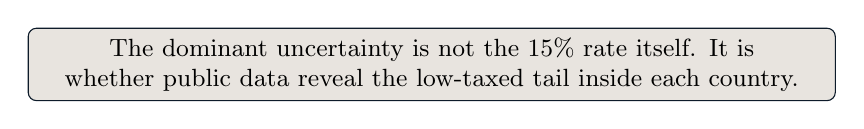
\begin{tikzpicture}[font=\small]
  \node[draw=Navy, rounded corners=3pt, fill=WarmGrey,
    minimum width=10.25cm, text width=9.65cm, minimum height=0.82cm, align=center] {
      The dominant uncertainty is not the 15\% rate itself. It is whether public data reveal the low-taxed tail inside each country.
    };
\end{tikzpicture}
\end{center}
\note{This slide can stand almost alone. The result is measurement, not a complicated tax-law claim.}
\end{frame}

\section{Behaviour}

\begin{frame}{Behavioural response: specification choice}
\small
\begin{columns}[T]
\begin{column}{0.39\textwidth}
\begin{block}{Reduced-form object}
  Reported profit is related to the effective tax rate within the same parent-affiliate relationship over time.
\end{block}
\begin{exampleblock}{Controls}
  Parent-affiliate fixed effects, year fixed effects, real activity controls and two-way clustered inference.
\end{exampleblock}
\end{column}
\begin{column}{0.57\textwidth}
\begin{center}
\scriptsize
\begin{tabular}{@{}L{2.55cm}rrr@{}}
  \toprule
  Specification & BIC rank & \(\Delta\)BIC & Tax Wald \(p\) \\
  \midrule
  Linear & 1 & 0.00 & \(1.5 \times 10^{-6}\) \\
  Logarithmic & 2 & 5.40 & \(1.2 \times 10^{-6}\) \\
  Quadratic & 3 & 7.54 & \(1.5 \times 10^{-6}\) \\
  \bottomrule
\end{tabular}
\end{center}

\vspace{0.25em}
\begin{center}
\scriptsize
\begin{tabular}{@{}L{2.55cm}rr@{}}
  \toprule
  ETR case & Semi-elasticity & Reallocation share \\
  \midrule
  Linear at 5\% & 1.50 & 13.9\% \\
  Linear at 10\% & 1.50 & 7.2\% \\
  Quadratic at 5\% & 1.72 & 15.4\% \\
  Logarithmic at 5\% & 2.00 & 16.5\% \\
  \bottomrule
\end{tabular}
\end{center}
\end{column}
\end{columns}

\vspace{0.15em}
\footnotesize
\emphbx{Reading:} the public CbCR panel supports a negative tax-profit relationship, but not sharp low-rate nonlinearity as the centre of the revenue answer.
\note{This is the statistics-facing slide. The important phrase is: the linear model is selected, not assumed.}
\end{frame}

\begin{frame}{Behavioural result in the revenue model}
\small
\begin{center}
\scriptsize
\begin{tabular}{@{}L{4.5cm}rL{4.0cm}@{}}
  \toprule
  Object & Estimate & Unit or reading \\
  \midrule
  Semi-elasticity & 1.50 & profit \% per pp ETR increase \\
  Reallocation at 5\% ETR & 13.9 & \% of reported profit \\
  Reallocation at 10\% ETR & 7.2 & \% of reported profit \\
  Revenue main effect & -46.7 & US\$ bn, 2017 to 2022 \\
  Scenario-variance main share & 5.1 & \% \\
  \bottomrule
\end{tabular}
\end{center}

\vspace{0.65em}
\begin{block}{Economic interpretation}
  The behavioural response is visible and meaningful, but it is not the main reason the revenue forecast moves across scenarios.
\end{block}
\note{Connect the regression directly to the decomposition. This is where the econometric result becomes policy-relevant.}
\end{frame}

\section{Substance and Allocation}

\begin{frame}{Substance result: 15\% is not the economic floor}
\small
\begin{center}
\scriptsize
\setlength{\tabcolsep}{3.5pt}
\begin{tabular}{@{}lrrrrr@{}}
  \toprule
  Group & SBIE (\%) & SBTI cap (\%) & Floor pre-SBTI (\%) & Floor post-SBTI (\%) & Change (pp) \\
  \midrule
  EU27 weighted & 10.4 & 3.7 & 14.2 & 11.9 & -2.3 \\
  Germany & 12.5 & 4.2 & 13.9 & 10.7 & -3.2 \\
  France & 12.6 & 5.8 & 13.8 & 10.2 & -3.6 \\
  Netherlands & 4.9 & 1.6 & 14.5 & 13.6 & -0.9 \\
  Ireland & 8.6 & 1.0 & 14.7 & 13.7 & -1.0 \\
  Luxembourg & 5.7 & 0.9 & 14.2 & 13.7 & -0.4 \\
  \bottomrule
\end{tabular}
\end{center}

\vspace{0.55em}
\begin{block}{Economic reading}
  The headline 15\% floor applies to excess profit, not to all profit. Payroll, tangible assets and substance-linked incentives lower the effective floor most where foreign-controlled activity is more capital intensive.
\end{block}
\note{This is the requested close-to-15-percent slide. Make clear that these are effective-floor results from the sectoral bridge, not observed safe-harbour claims.}
\end{frame}

\begin{frame}{Side-by-Side result: collection rights move}
\small
\begin{center}
\scriptsize
\setlength{\tabcolsep}{4pt}
\begin{tabular}{@{}L{2.7cm}C{2.25cm}C{2.45cm}L{3.45cm}@{}}
  \toprule
  Object & Universal (US\$ bn) & Side-by-Side (US\$ bn) & Effect \\
  \midrule
  Source-country collection & 282.5 & 282.5 & protected source revenue \\
  Residual backstop collection & 213.3 & 74.7 & -138.6 \\
  \midrule
  Total collector revenue & 495.8 & 357.2 & -138.6 \\
  \bottomrule
\end{tabular}
\end{center}

\vspace{0.45em}
\begin{columns}[T]
\begin{column}{0.48\textwidth}
\begin{alertblock}{Economic reading}
  Side-by-Side does not remove the low-taxed profit base. It removes residual collection rights for qualifying US-parented groups.
\end{alertblock}
\end{column}
\begin{column}{0.48\textwidth}
\begin{exampleblock}{Decomposition}
  The allocation regime explains \highlight{15.0\%} of pooled scenario variance and is the second-largest driver.
\end{exampleblock}
\end{column}
\end{columns}
\note{Do not show zero-change rows. Explain it as protected source-country revenue versus exposed residual backstop collection.}
\end{frame}

\section{Combined Results}

\begin{frame}{Revenue decomposition}
\small
\begin{center}
\scriptsize
\begin{tabular}{@{}L{2.55cm}C{1.85cm}C{2.05cm}L{4.55cm}@{}}
  \toprule
  Channel & Main share (\%) & Effect (US\$ bn) & Economic interpretation \\
  \midrule
  ETR measurement & 69.1 & +197.0 & the public data must identify the low-taxed mass inside jurisdictions \\
  Allocation rules & 15.0 & -87.5 & legal rules change where the tax accrues \\
  Behaviour & 5.1 & -46.7 & firms respond, but this is not the main forecast driver \\
  Substance shield & 4.6 & -43.6 & payroll and tangible assets reduce the effective floor \\
  Rate endpoint & 0.1 & +8.6 & transition rates matter little in the full design \\
  \bottomrule
\end{tabular}
\end{center}

\vspace{0.45em}
\begin{block}{Reading}
  Interactions explain 6.0\% of pooled scenario variance. The ranking still survives: measurement first, collection rights second, behaviour and substance smaller but economically visible.
\end{block}
\note{This is an important table-only slide. It is the synthesis of the thesis.}
\end{frame}

\begin{frame}{Stronger measurement windows}
\small
\begin{center}
\scriptsize
\setlength{\tabcolsep}{3.5pt}
\begin{tabular}{@{}L{3.35cm}rrrrL{2.6cm}@{}}
  \toprule
  Sample window & ETR (\%) & Allocation (\%) & Substance (\%) & Behaviour (\%) & Revenue range (US\$ bn) \\
  \midrule
  2017 to 2022 public panel & 72.0 & 16.6 & 5.7 & 5.5 & 127.7 to 517.4 \\
  2019 to 2022 stronger measurement & 80.3 & 11.4 & 4.5 & 3.7 & 73.0 to 332.4 \\
  2021 to 2022 strict overlap & 84.5 & 9.2 & 3.9 & 2.2 & 32.1 to 175.3 \\
  \bottomrule
\end{tabular}
\end{center}

\vspace{0.55em}
\begin{block}{Reading}
  When the window relies more directly on ETR-bracket evidence, measurement becomes an even larger share of the forecast spread. Preferred revenues are US\$303.7 bn, US\$193.0 bn and US\$102.3 bn respectively.
\end{block}
\note{This slide clarifies the difference between ANOVA main share and Shapley allocated shares.}
\end{frame}

\begin{frame}{Country policy readings}
\small
\begin{center}
\scriptsize
\setlength{\tabcolsep}{3.5pt}
\begin{tabular}{@{}lrrrrL{2.25cm}@{}}
  \toprule
  Country & Rev. (US\$ bn) & Rev./CIT (\%) & Spread/CIT (\%) & Domestic (\%) & Dominant channel \\
  \midrule
  Germany & 44.5 & 9.0 & 16.2 & 55.4 & measurement \\
  Netherlands & 87.1 & 41.4 & 38.5 & 92.2 & measurement \\
  France & 20.2 & 5.4 & 12.6 & 58.5 & measurement \\
  Luxembourg & 51.7 & 225.1 & 181.7 & 92.6 & legal allocation \\
  Ireland & 27.1 & 30.3 & 29.7 & 86.0 & substance \\
  Hungary & 3.9 & 26.8 & 40.2 & 88.0 & measurement \\
  \bottomrule
\end{tabular}
\end{center}

\vspace{0.45em}
\begin{alertblock}{Policy reading}
  A finance ministry should not rank cases by revenue alone. Fiscal salience, uncertainty and domestic collection exposure point to different priorities.
\end{alertblock}
\note{This replaces the abstract country typology with numbers.}
\end{frame}

\begin{frame}{Policy next steps}
\footnotesize
\begin{columns}[T]
\begin{column}{0.48\textwidth}
\begin{block}{1. Distributional ETR data}
  Report profit and tax by ETR bands below 15\%. This is the largest forecast driver.
\end{block}
\end{column}
\begin{column}{0.48\textwidth}
\begin{exampleblock}{2. Domestic collection capacity}
  Monitor domestic coverage and residual exposure. Allocation changes fiscal incidence.
\end{exampleblock}
\end{column}
\end{columns}

\vspace{0.35em}
\begin{columns}[T]
\begin{column}{0.48\textwidth}
\begin{block}{3. Forecast governance}
  Publish scenario decompositions, not only one budget number. The range is economically large.
\end{block}
\end{column}
\begin{column}{0.48\textwidth}
\begin{alertblock}{4. Ex-post validation}
  Compare forecasts with observed collections once implementation data become available.
\end{alertblock}
\end{column}
\end{columns}

\vspace{0.45em}
\begin{block}{Policy implication}
  Highest-return improvement: better distributional measurement, followed by transparent collection-right modelling.
\end{block}
\note{This is the practical policy answer. It should sound like advice to policymakers.}
\end{frame}

\begin{frame}{Conclusion}
\small
\begin{center}
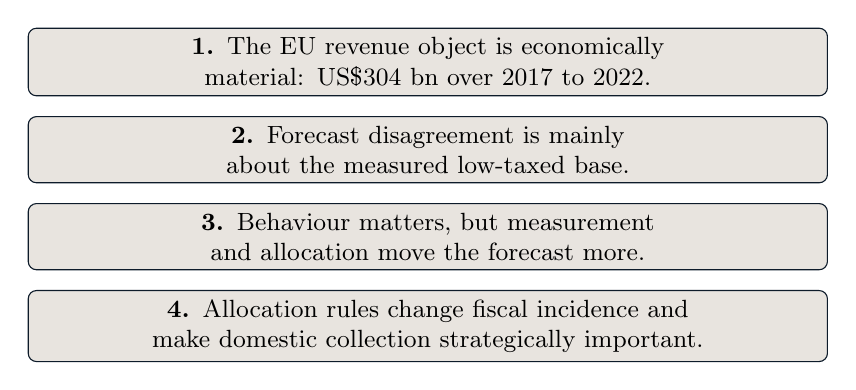
\begin{tikzpicture}[font=\small, node distance=0.38cm]
  \tikzset{
    point/.style={draw=Navy, rounded corners=3pt, fill=WarmGrey,
      minimum width=10.15cm, text width=9.55cm, minimum height=0.70cm, align=center}
  }
  \node[point] (p1) {\textbf{1.} The EU revenue object is economically material: \USD304 bn over 2017 to 2022.};
  \node[point, below=0.25cm of p1] (p2) {\textbf{2.} Forecast disagreement is mainly about the measured low-taxed base.};
  \node[point, below=0.25cm of p2] (p3) {\textbf{3.} Behaviour matters, but measurement and allocation move the forecast more.};
  \node[point, below=0.25cm of p3] (p4) {\textbf{4.} Allocation rules change fiscal incidence and make domestic collection strategically important.};
\end{tikzpicture}
\end{center}

\vspace{0.45em}
\centering
\highlight{The thesis contributes an economic policy decomposition of a contested fiscal forecast.}
\note{End with the contribution, not with limitations.}
\end{frame}

{
\setbeamercolor{background canvas}{bg=Navy}
\begin{frame}[plain]
  \vspace{1.45em}
  \begin{center}
    {\color{Ivory}\Large\bfseries Thank you}\\[1.15em]
    {\color{DkOrange}\rule{4.2cm}{2pt}}\\[1.15em]
    {\color{WarmGrey}\normalsize Measurement defines the base.}\\[0.38em]
    {\color{LtOrange}\normalsize Behaviour calibrates the response.}\\[0.38em]
    {\color{WarmGrey}\normalsize Collection rights determine fiscal incidence.}\\[1.25em]
    {\color{MidGrey}\small Maurits de Haan $\cdot$ m.c.p.dehaan@students.uu.nl}
  \end{center}
\end{frame}
}

\appendix

{
\setbeamercolor{background canvas}{bg=MidNavy}
\begin{frame}[plain]
  \vfill
  \centering
  {\color{Ivory}\LARGE\bfseries Backup slides}\\[0.6em]
  {\color{DkOrange}\rule{4cm}{2pt}}\\[0.8em]
  {\color{WarmGrey}\small Use only when asked for the technical detail.}
  \vfill
\end{frame}
}

\begin{frame}{Backup: acronyms and collection rule}
\small
\begin{center}
\scriptsize
\begin{tabular}{@{}L{2.25cm}L{4.25cm}L{4.8cm}@{}}
  \toprule
  \textbf{Term} & \textbf{Plain meaning} & \textbf{Revenue role} \\
  \midrule
  QDMTT & qualified domestic minimum top-up tax & source country collects first \\
  IIR & income inclusion rule & parent country collects if source country does not \\
  UTPR & undertaxed profits rule & implementing countries collect residual backstop revenue \\
  Side-by-Side & safe harbour for qualifying parent regimes in the thesis model & residual IIR and UTPR set to zero for qualifying US-parented groups \\
  SBIE & substance-based income exclusion & payroll and tangible assets shield part of the base \\
  SBTI & substance-based tax incentive safe harbour & capacity for substance-linked incentives to be protected \\
  \bottomrule
\end{tabular}
\end{center}
\sourceline{thesisv4 Sections 3 and 4}
\end{frame}

\begin{frame}{Backup: source hierarchy for Stage 1}
\small
\begin{center}
\scriptsize
\begin{tabular}{@{}lrrrrrrr@{}}
  \toprule
  Source & 2017 & 2018 & 2019 & 2020 & 2021 & 2022 & Total \\
  \midrule
  Direct Table IV & 0 & 0 & 2,275 & 2,306 & 2,470 & 2,344 & 9,395 \\
  Beta percentile fit & 0 & 0 & 0 & 0 & 421 & 399 & 820 \\
  BSPI shape transport & 1,720 & 2,179 & 0 & 0 & 0 & 0 & 3,899 \\
  Jurisdiction-average fallback & 303 & 348 & 393 & 408 & 5 & 2 & 1,459 \\
  Missing source & 22 & 27 & 43 & 36 & 25 & 32 & 185 \\
  \bottomrule
\end{tabular}
\end{center}
\begin{block}{Interpretation}
  Direct Table IV carries the main distributional branch after 2019. The early years require shape transport, which is why the robustness slides restrict the window.
\end{block}
\sourceline{generated Table stage1\_source\_coverage}
\end{frame}

\begin{frame}{Backup: profit-base correction}
\small
\begin{columns}[T]
\begin{column}{0.48\textwidth}
\begin{center}
\scriptsize
\begin{tabular}{@{}lrr@{}}
  \toprule
  Profit branch & Reported & Corrected \\
  \midrule
  OECD adjusted & 851.0 & 609.2 \\
  External-anchor domestic & 5,308.8 & 2,491.1 \\
  Domestic model & 24,642.7 & 15,831.7 \\
  Foreign affiliates & 15,908.8 & 15,908.8 \\
  \midrule
  Total & 46,711.2 & 34,840.8 \\
  \bottomrule
\end{tabular}
\end{center}
\tiny Current US\$ bn.
\end{column}
\begin{column}{0.48\textwidth}
\begin{block}{Why it matters}
  The correction addresses double-counting exposure in domestic parent cells. It reduces positive-profit CbCR profit by 25.4\% before any GMT revenue stage is estimated.
\end{block}
\begin{alertblock}{Interpretive boundary}
  This is a denominator correction, not a claim about new tax payments.
\end{alertblock}
\end{column}
\end{columns}
\sourceline{generated Table profit\_correction\_effects}
\end{frame}

\begin{frame}{Backup: annual Stage 1 rates}
\small
\begin{center}
\scriptsize
\begin{tabular}{@{}lrrrrrr@{}}
  \toprule
  EU27 & 2017 & 2018 & 2019 & 2020 & 2021 & 2022 \\
  \midrule
  Average rule, low-taxed share & 53.9 & 63.3 & 62.5 & 55.0 & 55.3 & 41.8 \\
  Average rule, liability rate & 3.5 & 4.6 & 3.8 & 2.9 & 2.9 & 1.4 \\
  Distributional rule, low-taxed share & 52.3 & 55.6 & 53.4 & 50.9 & 51.5 & 43.8 \\
  Distributional rule, liability rate & 5.8 & 6.1 & 5.7 & 4.8 & 4.9 & 3.7 \\
  \bottomrule
\end{tabular}
\end{center}
\begin{block}{Reading}
  The distributional branch usually does not raise the low-taxed share dramatically. It raises the liability rate because the identified low-taxed slice has a larger average top-up gap.
\end{block}
\sourceline{generated Table stage1\_rates}
\end{frame}

\begin{frame}{Backup: behavioural regression output}
\small
\begin{center}
\scriptsize
\begin{tabular}{@{}lccc@{}}
  \toprule
  & Linear & Quadratic & Logarithmic \\
  \midrule
  ETR & -1.500*** (0.272) & -1.761* (0.909) & -0.943 (0.973) \\
  ETR squared & & 0.438 (1.262) & \\
  Log shifted ETR & & & -0.214 (0.415) \\
  Log tangible assets & -0.017 (0.015) & -0.017 (0.015) & -0.017 (0.015) \\
  Log payroll proxy & 0.023 (0.034) & 0.023 (0.034) & 0.023 (0.034) \\
  \midrule
  $N$ & 8,971 & 8,971 & 8,971 \\
  Parent-affiliate pairs & 1,936 & 1,936 & 1,936 \\
  BIC rank & 1 & 3 & 2 \\
  $\Delta$BIC & 0.00 & 7.54 & 5.40 \\
  \bottomrule
\end{tabular}
\end{center}
\tiny All models include parent-affiliate and year fixed effects. Standard errors are two-way clustered by parent and affiliate.
\sourceline{generated Table stage3\_regression\_table}
\end{frame}

\begin{frame}{Backup: behavioural reliability scorecard}
\small
\begin{center}
\scriptsize
\begin{tabular}{@{}L{3.3cm}L{4.2cm}L{4.2cm}@{}}
  \toprule
  Diagnostic & Result & Weight for interpretation \\
  \midrule
  Preferred FE estimate & semi-elasticity 1.50; $N=8,971$; pairs $=1,936$ & usable scenario coefficient \\
  Model selection & BIC selects linear; tax Wald $p=1.5\times10^{-6}$ & supports parsimonious response \\
  Two-way inference & SE $=0.272$; $p=1.5\times10^{-6}$ & statistically strong association \\
  IV diagnostics & first stages relevant; 2SLS imprecise & weak for causal replacement \\
  Low-ETR tail & below 5\% ETR: 17.4\% of rows & tail exists but does not prove curvature \\
  Final decision & use as scenario coefficient & do not make it causal centrepiece \\
  \bottomrule
\end{tabular}
\end{center}
\sourceline{generated Table stage3\_reliability\_scorecard}
\end{frame}

\begin{frame}{Backup: Stage 1 measurement-error interval}
\small
\begin{center}
\scriptsize
\begin{tabular}{@{}llrrrrr@{}}
  \toprule
  Behaviour & Regime & Baseline & Median & 5th pct. & 95th pct. & 90\% width \\
  \midrule
  Mechanical & Universal & 495.8 & 468.6 & 399.3 & 542.6 & 143.3 \\
  Mechanical & SbS & 357.2 & 342.0 & 297.8 & 391.5 & 93.7 \\
  Behavioural & Universal & 421.8 & 394.6 & 336.5 & 456.5 & 120.1 \\
  Behavioural & SbS & 303.7 & 287.5 & 250.8 & 329.3 & 78.6 \\
  \bottomrule
\end{tabular}
\end{center}
\tiny US\$ bn. Intervals use centred empirical residuals from the Table I percentile-fit versus Table IV overlap.
\begin{block}{Reading}
  Even inside the preferred scenario, measurement error in Stage 1 remains a material forecast object.
\end{block}
\sourceline{generated Table stage1\_measurement\_error\_interval}
\end{frame}

\begin{frame}{Backup: Shapley allocation after interactions}
\small
\begin{center}
\scriptsize
\begin{tabular}{@{}L{2.8cm}L{4.0cm}rrr@{}}
  \toprule
  Factor & Mechanism & Main & Interaction & Allocated \\
  \midrule
  ETR measurement & low-taxed profit base & 69.1 & 2.9 & 72.0 \\
  Side-by-Side regime & legal allocation & 15.0 & 1.6 & 16.6 \\
  Substance specification & substance shield & 4.6 & 1.1 & 5.7 \\
  Behavioural response & response coefficient & 5.1 & 0.4 & 5.5 \\
  SBIE rate endpoint & policy parameter & 0.1 & 0.0 & 0.2 \\
  \bottomrule
\end{tabular}
\end{center}
\begin{block}{Reading}
  The same ranking survives when interactions are split across the factors that generate them.
\end{block}
\sourceline{generated Table stage4\_6\_shapley\_factor\_attribution}
\end{frame}

\begin{frame}{Backup: selected country spreads}
\small
\begin{columns}[T]
\begin{column}{0.48\textwidth}
\begin{center}
\scriptsize
\begin{tabular}{@{}lrrr@{}}
  \toprule
  Country & Minimum & Maximum & Spread \\
  \midrule
  Germany & 3.3 & 83.2 & 79.9 \\
  Netherlands & 42.7 & 123.7 & 81.0 \\
  France & 0.9 & 48.3 & 47.4 \\
  Luxembourg & 45.9 & 87.6 & 41.7 \\
  Ireland & 18.6 & 45.2 & 26.6 \\
  Hungary & 0.3 & 6.1 & 5.8 \\
  \bottomrule
\end{tabular}
\end{center}
\tiny US\$ bn, 2017 to 2022.
\end{column}
\begin{column}{0.48\textwidth}
\begin{block}{Reading}
  Germany and the Netherlands have similar absolute spreads, but different policy readings. Germany is mainly a measurement case; the Netherlands is largely protected through QDMTT collection.
\end{block}
\begin{alertblock}{Luxembourg}
  The estimate is best read as a fiscal stress statistic, not as ordinary budgetable cash.
\end{alertblock}
\end{column}
\end{columns}
\sourceline{generated Tables country\_spread and country\_fiscal\_salience}
\end{frame}

\begin{frame}{Backup: fiscal salience of selected countries}
\small
\begin{center}
\scriptsize
\begin{tabular}{@{}lrrrrr@{}}
  \toprule
  Country & Revenue & Revenue/CIT & Spread/CIT & SbS loss/CIT & QDMTT/revenue \\
  \midrule
  Germany & 44.5 & 9.0\% & 16.2\% & 4.7\% & 55.4\% \\
  Netherlands & 87.1 & 41.4\% & 38.5\% & 6.0\% & 92.2\% \\
  France & 20.2 & 5.4\% & 12.6\% & 5.0\% & 58.5\% \\
  Luxembourg & 51.7 & 225.1\% & 181.7\% & 77.4\% & 92.6\% \\
  Ireland & 27.1 & 30.3\% & 29.7\% & 13.7\% & 86.0\% \\
  Hungary & 3.9 & 26.8\% & 40.2\% & 7.3\% & 88.0\% \\
  \bottomrule
\end{tabular}
\end{center}
\tiny Revenue is preferred behavioural Side-by-Side collector-country revenue, US\$ bn.
\sourceline{generated Table country\_fiscal\_salience}
\end{frame}

\begin{frame}{Backup: SBTI capital-intensity regression}
\small
\begin{columns}[T]
\begin{column}{0.48\textwidth}
\begin{center}
\scriptsize
\resizebox{\linewidth}{!}{%
\begin{tabular}{@{}lrrrr@{}}
  \toprule
  Specification & Coefficient & SE & $p$ & $R^2$ \\
  \midrule
  Unweighted & -0.00008 & 0.00003 & 0.026 & 0.386 \\
  Profit-weighted & -0.00162 & 0.00045 & 0.001 & 0.484 \\
  \bottomrule
\end{tabular}
}
\end{center}
\end{column}
\begin{column}{0.48\textwidth}
\begin{block}{Interpretation}
  Higher tangible-asset intensity is associated with a larger SBTI-induced reduction in the effective floor.
\end{block}
\begin{alertblock}{Caveat}
  The dependent variable is exposure capacity in public data, not observed safe-harbour elections.
\end{alertblock}
\end{column}
\end{columns}
\sourceline{generated Table stage2\_h5\_regression}
\end{frame}

\begin{frame}{Backup: literature anchors}
\small
\begin{center}
\scriptsize
\begin{tabular}{@{}L{3.2cm}L{7.6cm}@{}}
  \toprule
  Literature & Role in the thesis \\
  \midrule
  Hines and Rice (1994) & reported profit responds to tax incentives after controlling for real activity \\
  Heckemeyer and Overesch (2017) & meta-regression benchmark for profit-shifting semi-elasticities \\
  Dowd et al. (2017) & nonlinear low-rate response benchmark \\
  Garcia-Bernardo et al. (2024) & logarithmic behavioural specification and formulary reallocation logic \\
  Blouin and Robinson (2023) & double-counting risk in profit-shifting estimates \\
  Hugger et al. (2026) & low-taxed mass can sit inside above-average-ETR jurisdictions \\
  Devereux et al. (2023); Schjelderup (2024) & substance carve-outs lower the effective floor and can resemble production subsidies \\
  \bottomrule
\end{tabular}
\end{center}
\sourceline{thesisv4 Literature review and bibliography}
\end{frame}

\end{document}
